% 
% Annual Cognitive Science Conference
% Sample LaTeX Paper -- Proceedings Format
% 

% Original : Ashwin Ram (ashwin@cc.gatech.edu)       04/01/1994
% Modified : Johanna Moore (jmoore@cs.pitt.edu)      03/17/1995
% Modified : David Noelle (noelle@ucsd.edu)          03/15/1996
% Modified : Pat Langley (langley@cs.stanford.edu)   01/26/1997
% Latex2e corrections by Ramin Charles Nakisa        01/28/1997 
% Modified : Tina Eliassi-Rad (eliassi@cs.wisc.edu)  01/31/1998
% Modified : Trisha Yannuzzi (trisha@ircs.upenn.edu) 12/28/1999 (in process)
% Modified : Mary Ellen Foster (M.E.Foster@ed.ac.uk) 12/11/2000
% Modified : Ken Forbus                              01/23/2004
% Modified : Eli M. Silk (esilk@pitt.edu)            05/24/2005
% Modified: Niels Taatgen (taatgen@cmu.edu)  10/24/2006

%% Change ``a4paper'' in the following line to ``letterpaper'' if you are
%% producing a letter-format document.

\documentclass[10pt,letterpaper]{article}

\usepackage{cogsci}
\usepackage{pslatex}
\usepackage{apacite}
\usepackage{graphicx}

\title{ Counterfactual Distance (?) }
 
\author{{\large \bf Desmond C. Ong (dco@stanford.edu)} \\
{\large \bf Jamil Zaki (jzaki@stanford.edu)} \\
{\large \bf Noah D. Goodman (ngoodman@stanford.edu)} \\
  Department of Psychology, Stanford University, Stanford CA, USA 
}

%array of cards
%choose card
%winning card is either proximally closer or numerically closer

%proximally closer vs numerically closer vs different suit (diamond & heart vs. spade & club)
% 3 forced choice (A, B, or equal)

% die + card task

\begin{document}

\maketitle

\begin{abstract}
abstract text

\textbf{Keywords:} 
Near Miss; Counterfactual Distance; Lay Theories; Emotion
\end{abstract}


\begin{quote}
\textit{``Close only counts in horseshoes and hand grenades"} 
-- English Idiom
\end{quote}

	Argentina nearly won the 2014 FIFA World Cup Final, conceding the only goal of the match with barely 7 minutes left in extra time, but as the above idiom morbidly points out\footnote{Points in horseshoes are scored based on distance thrown horseshoes land from the target stake. Thrown hand grenades, in contrast, do not need to hit their target to be effective.}, close in this case, does not count. However close they were, they did not win. However, as Argentinian supporters would attest, close does matter---\textit{emotionally}.

	Though we live in only one of many possible realizations of the world, our mental lives---and consequently, our emotional lives---are constantly spent exploring other possible worlds via counterfactual thinking \cite{Bryne2002, Gleicher1990, Johnson1986, Roese1997}. ``Near-miss" or close counterfactual comparisons in particular, are so mentally engaging because these possible worlds had almost happened. Consider \citeA{Kahneman1982}'s classic example of missing a plane by 5 minutes, as opposed to 30 minutes: people consistently and reliably judge the person who narrowly missed his plane to feel much worse than the one who missed it by a wider margin. One proposed reason is that it is much easier to generate possible counterfactual antecedents that would have resulted in the counterfactual consequent of catching the plane. The near-miss character could easily generate counterfactuals like ``If only I woke up 5 minutes earlier" or ``if only I had packed my bag the night before", that would result in the consequent ``then I would have caught my plane". If the counterfactual world is somehow \textit{closer} to the current world, then perhaps the counterfactual world would only require a smaller change in the causal chain that led up to the current world in order to be realized.

	Previous research has identified some of the impact of closeness on counterfactual thought \cite{Kahneman1990, Teigen1996}. Closeness increases the activation of counterfactual thought, by increasing the salience of the counterfactual world \cite{Kahneman1982, Roese1997}, and additionally also amplifies the affective consequence of the counterfactual comparison \cite{Johnson1986, Kahneman1982}. Narrowly missing a plane or a World Cup Title feels far worse than missing it by a large margin. Yet, there remains many open questions regarding the nature of these distances. What are the relevant dimensions of closeness that people incorporate into their lay theories of the world, and into their lay theories of emotion?
	
	

\subsection{Outline of paper:}
\begin{enumerate}
\item Lay out near miss predictions. Noticably: clearly, on both win and lose sides.
\item Expt 1: just show it with vignettes, where distance is causally related to outcome
\item Expt 2: show it with die vignettes, where distance is irrelevant
\item Expt 3: card task, show that the relevant dimension can be tweaked
\end{enumerate}

\section{Predictions}


\begin{figure}[htb!]
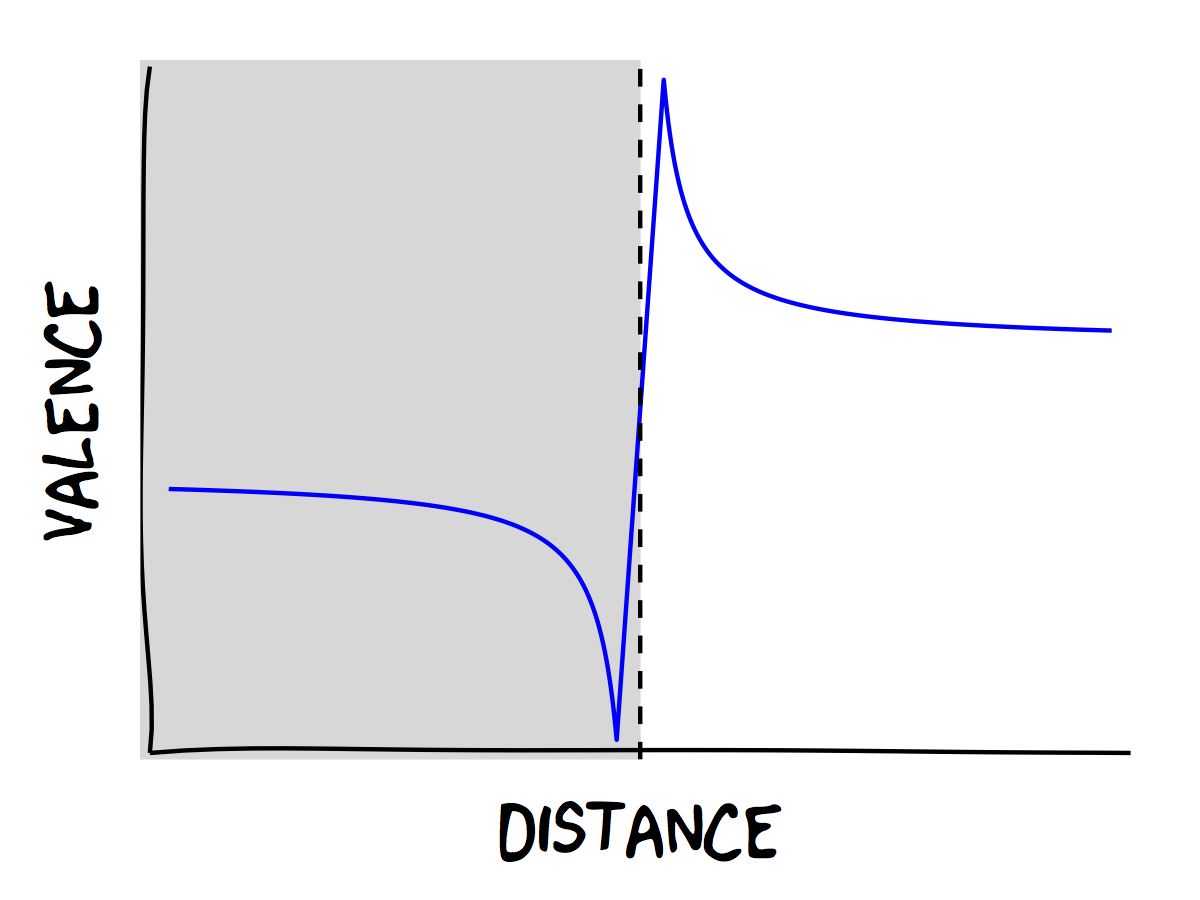
\includegraphics[width=\columnwidth]{images/predictionFig.png}
\caption{ Prediction. Will tweak labels.}
\label{PredictionFig}
\end{figure}

\newpage
\section{Experiment 1: Vignettes}


\begin{figure}[htb!]
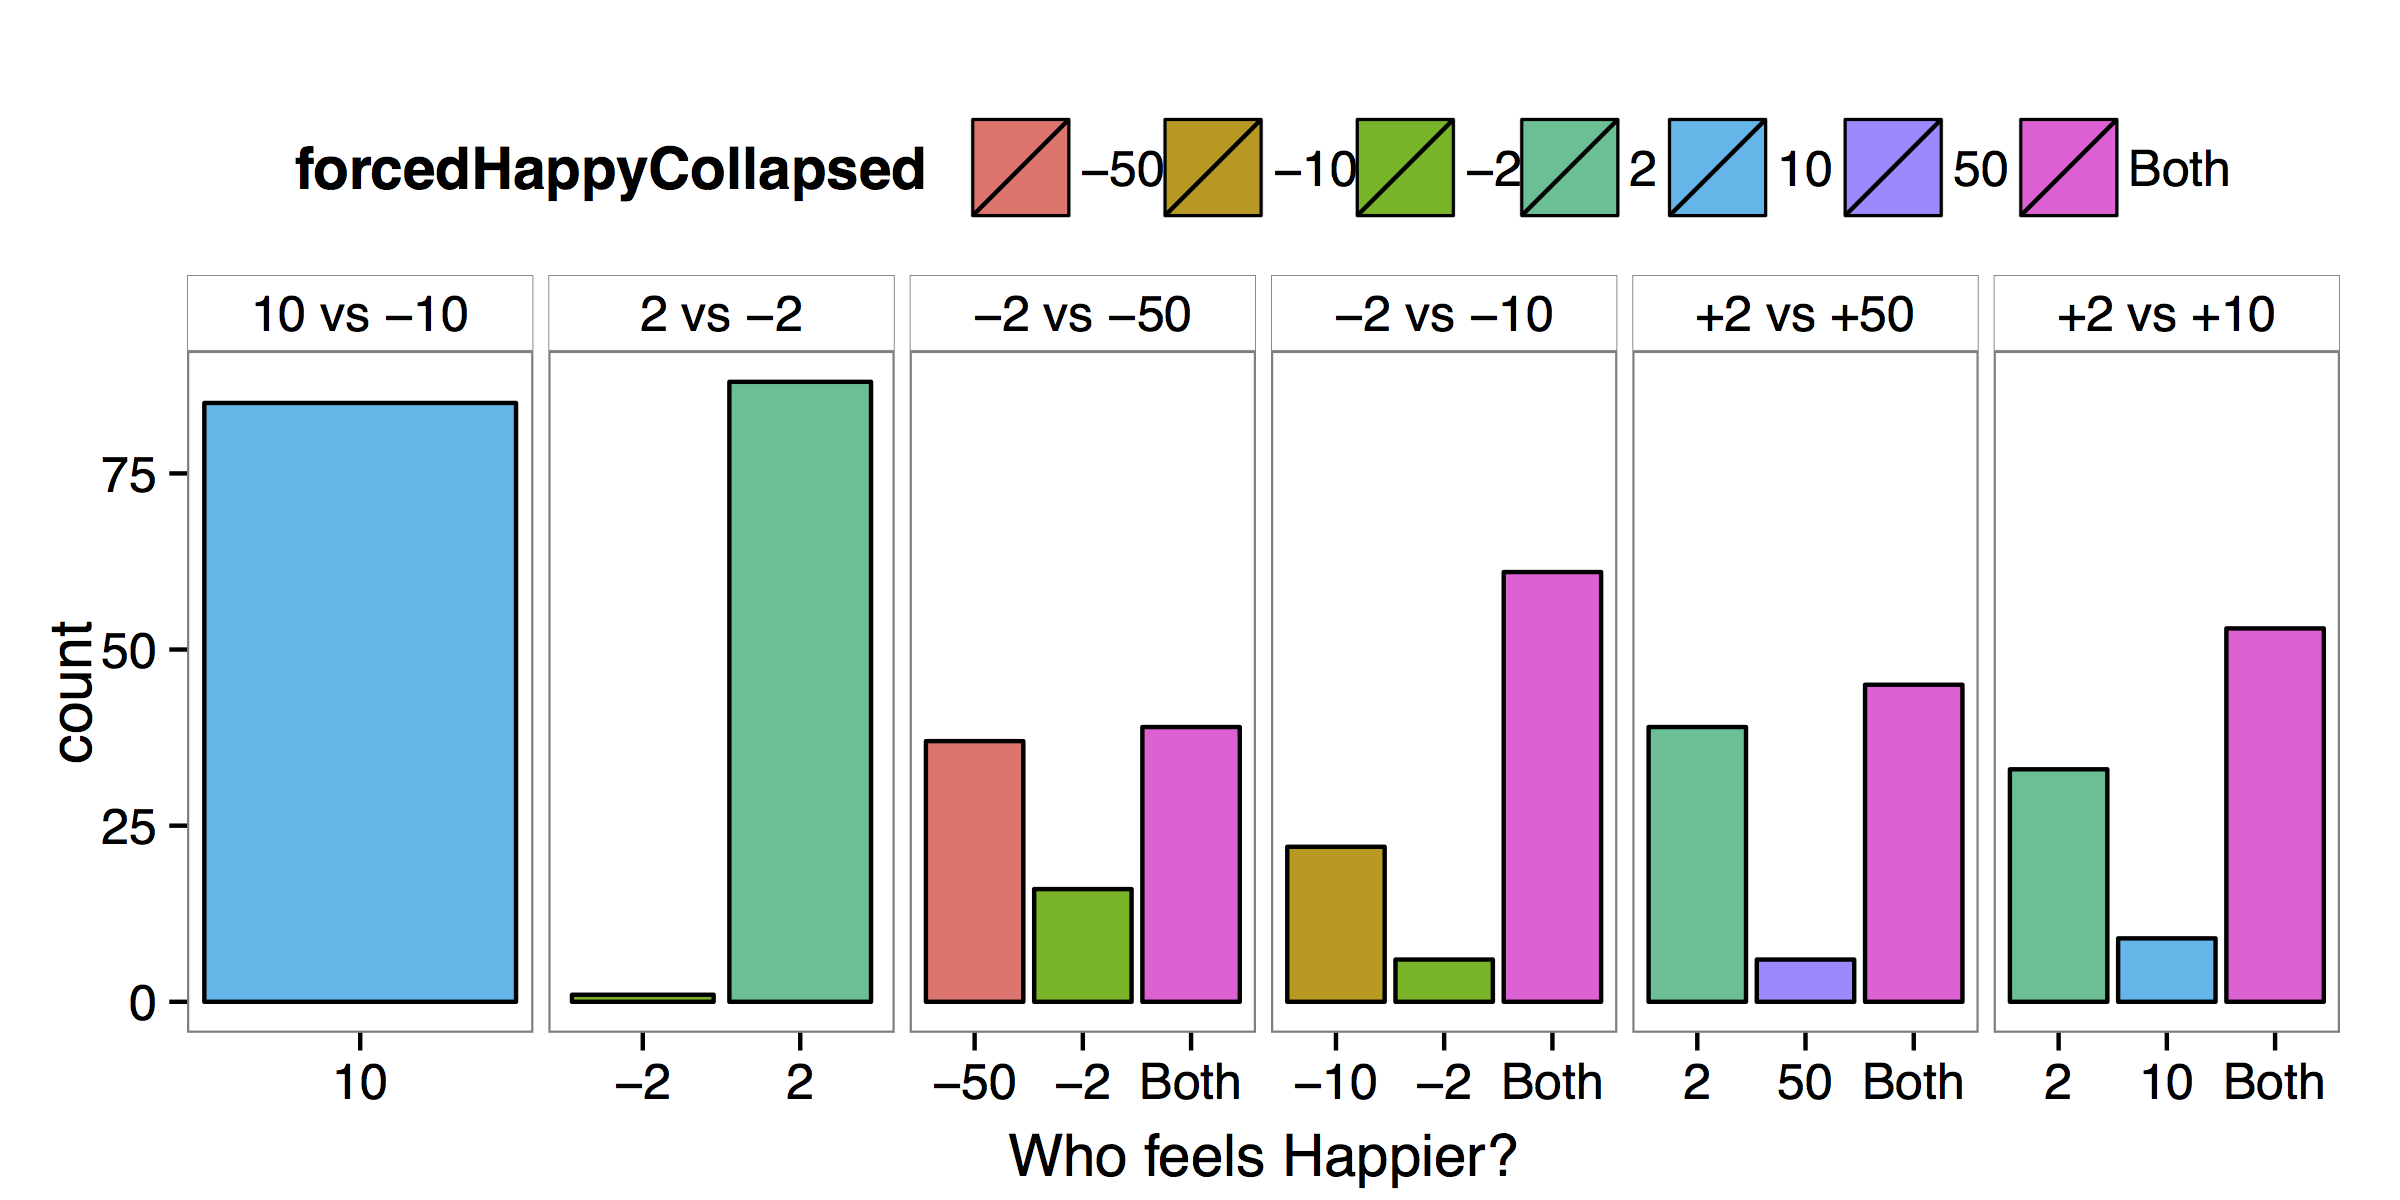
\includegraphics[width=\columnwidth]{images/vignettes_forcedHappy.png}
\caption{ Expt 1 Results. Will make this bigger.}
\label{Expt1ResultFig}
\end{figure}


\section{Experiment 2: Dice vignette}



\begin{figure}[htb!]
%\includegraphics[width=\columnwidth]{images/expt2results.png}
\caption{ Expt 2 Results.}
\label{Expt2ResultFig}
\end{figure}


\section{Experiment 3: Card task}


\begin{figure}[htb!]
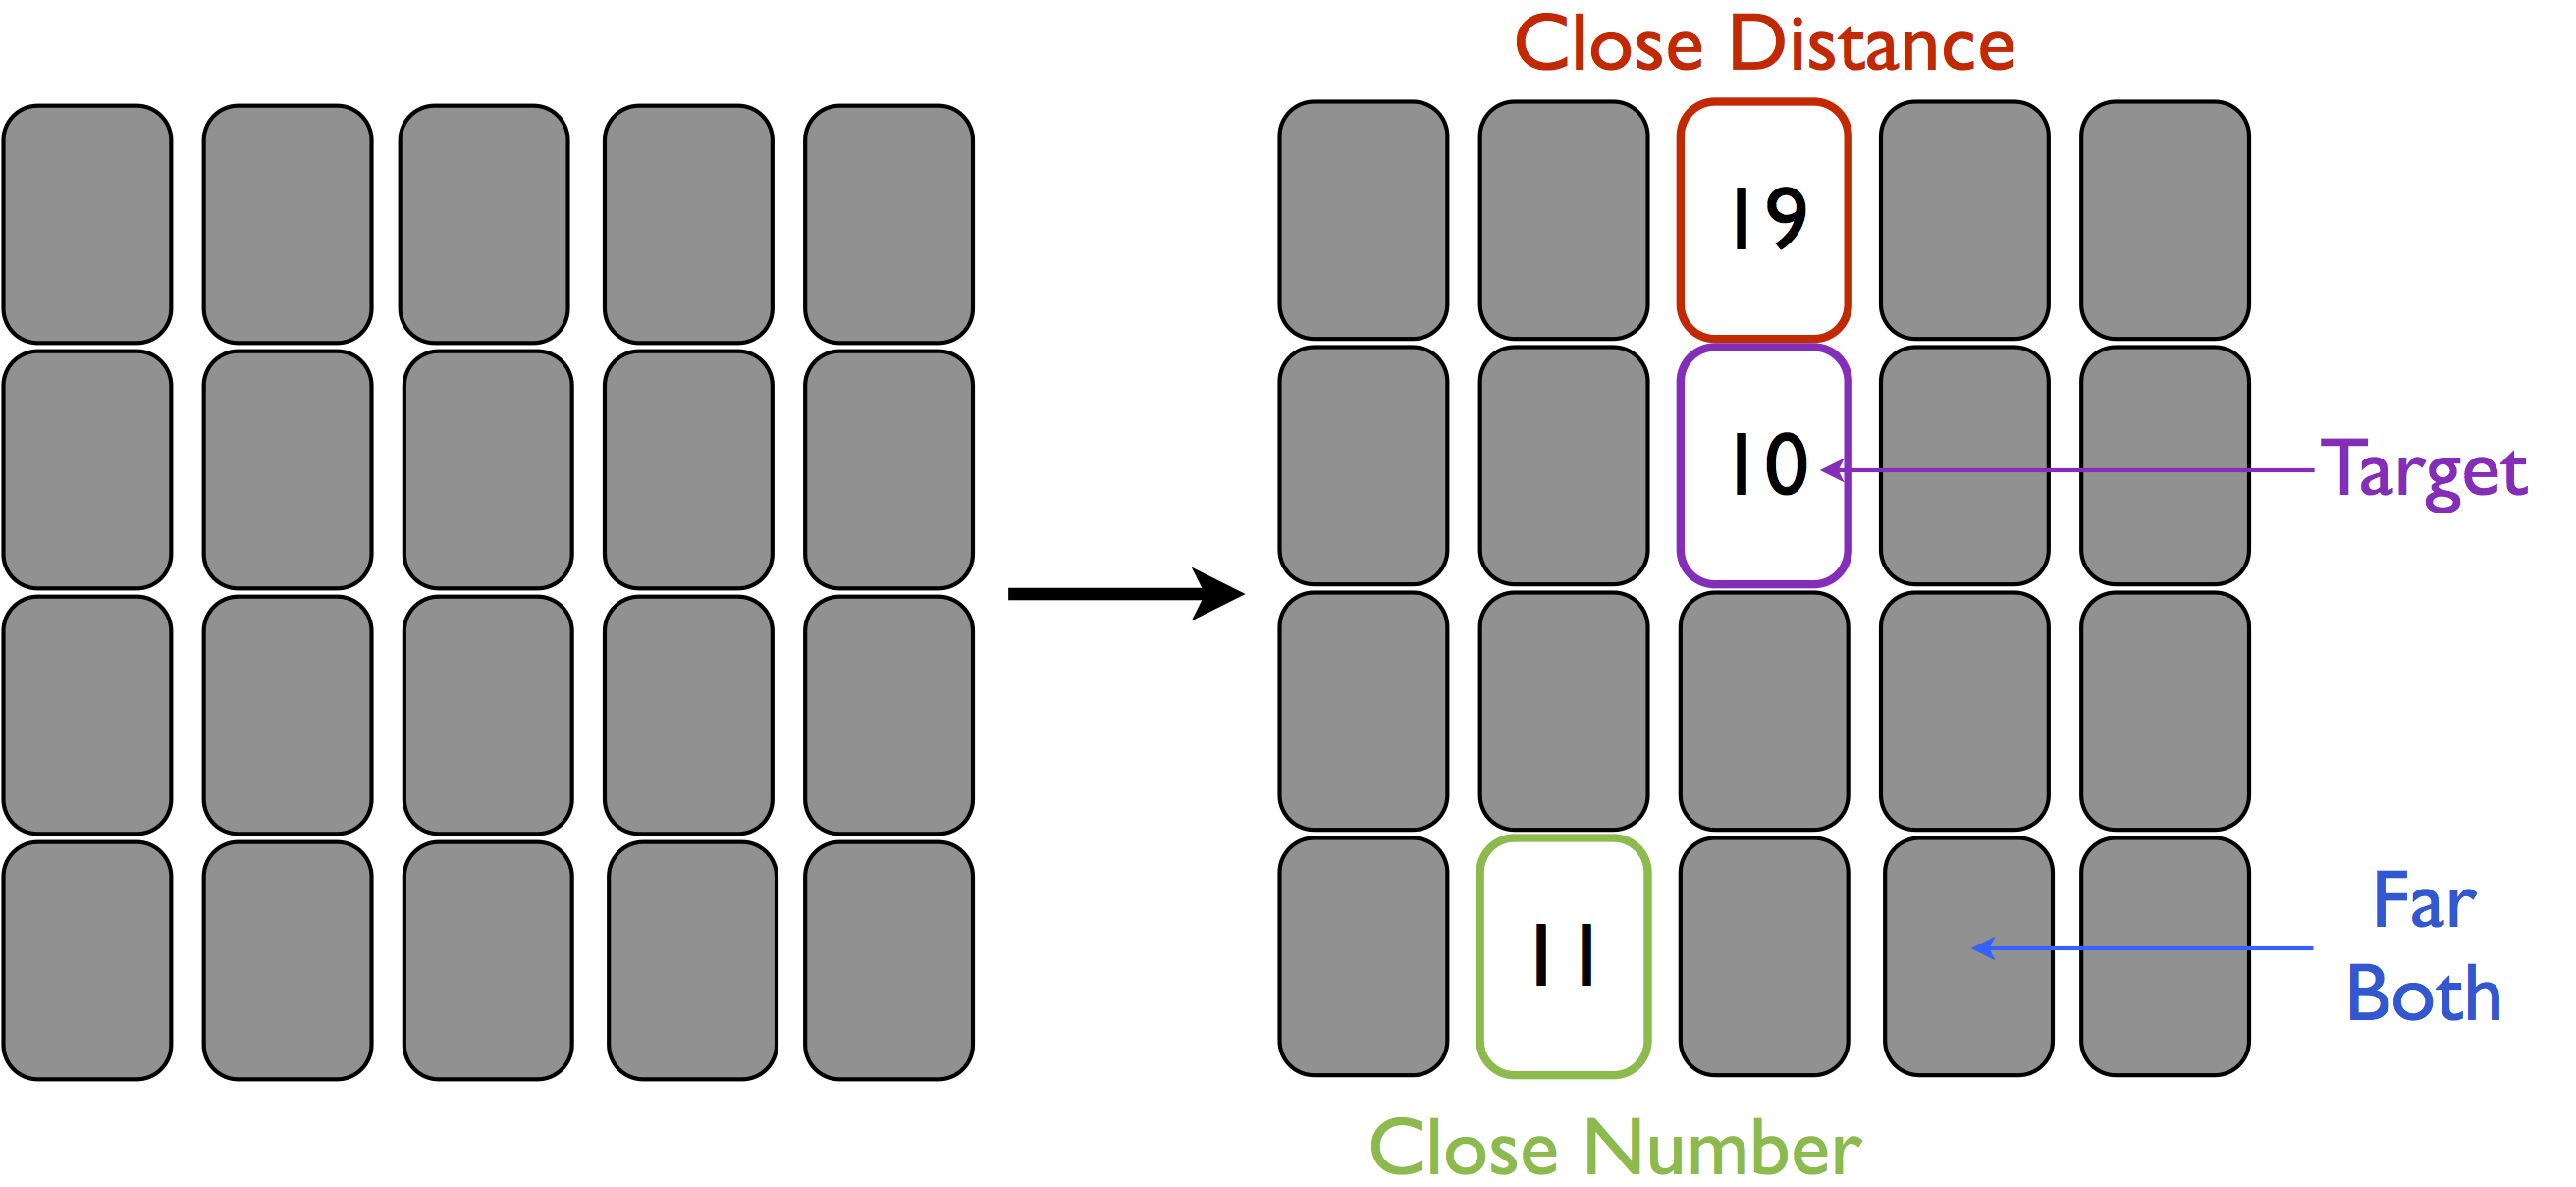
\includegraphics[width=\columnwidth]{images/card_paradigm.png}
\caption{ Expt 3 Paradigm. Will make this smaller. }
\label{Expt3ParadigmFig}
\end{figure}

\begin{figure}[htb!]
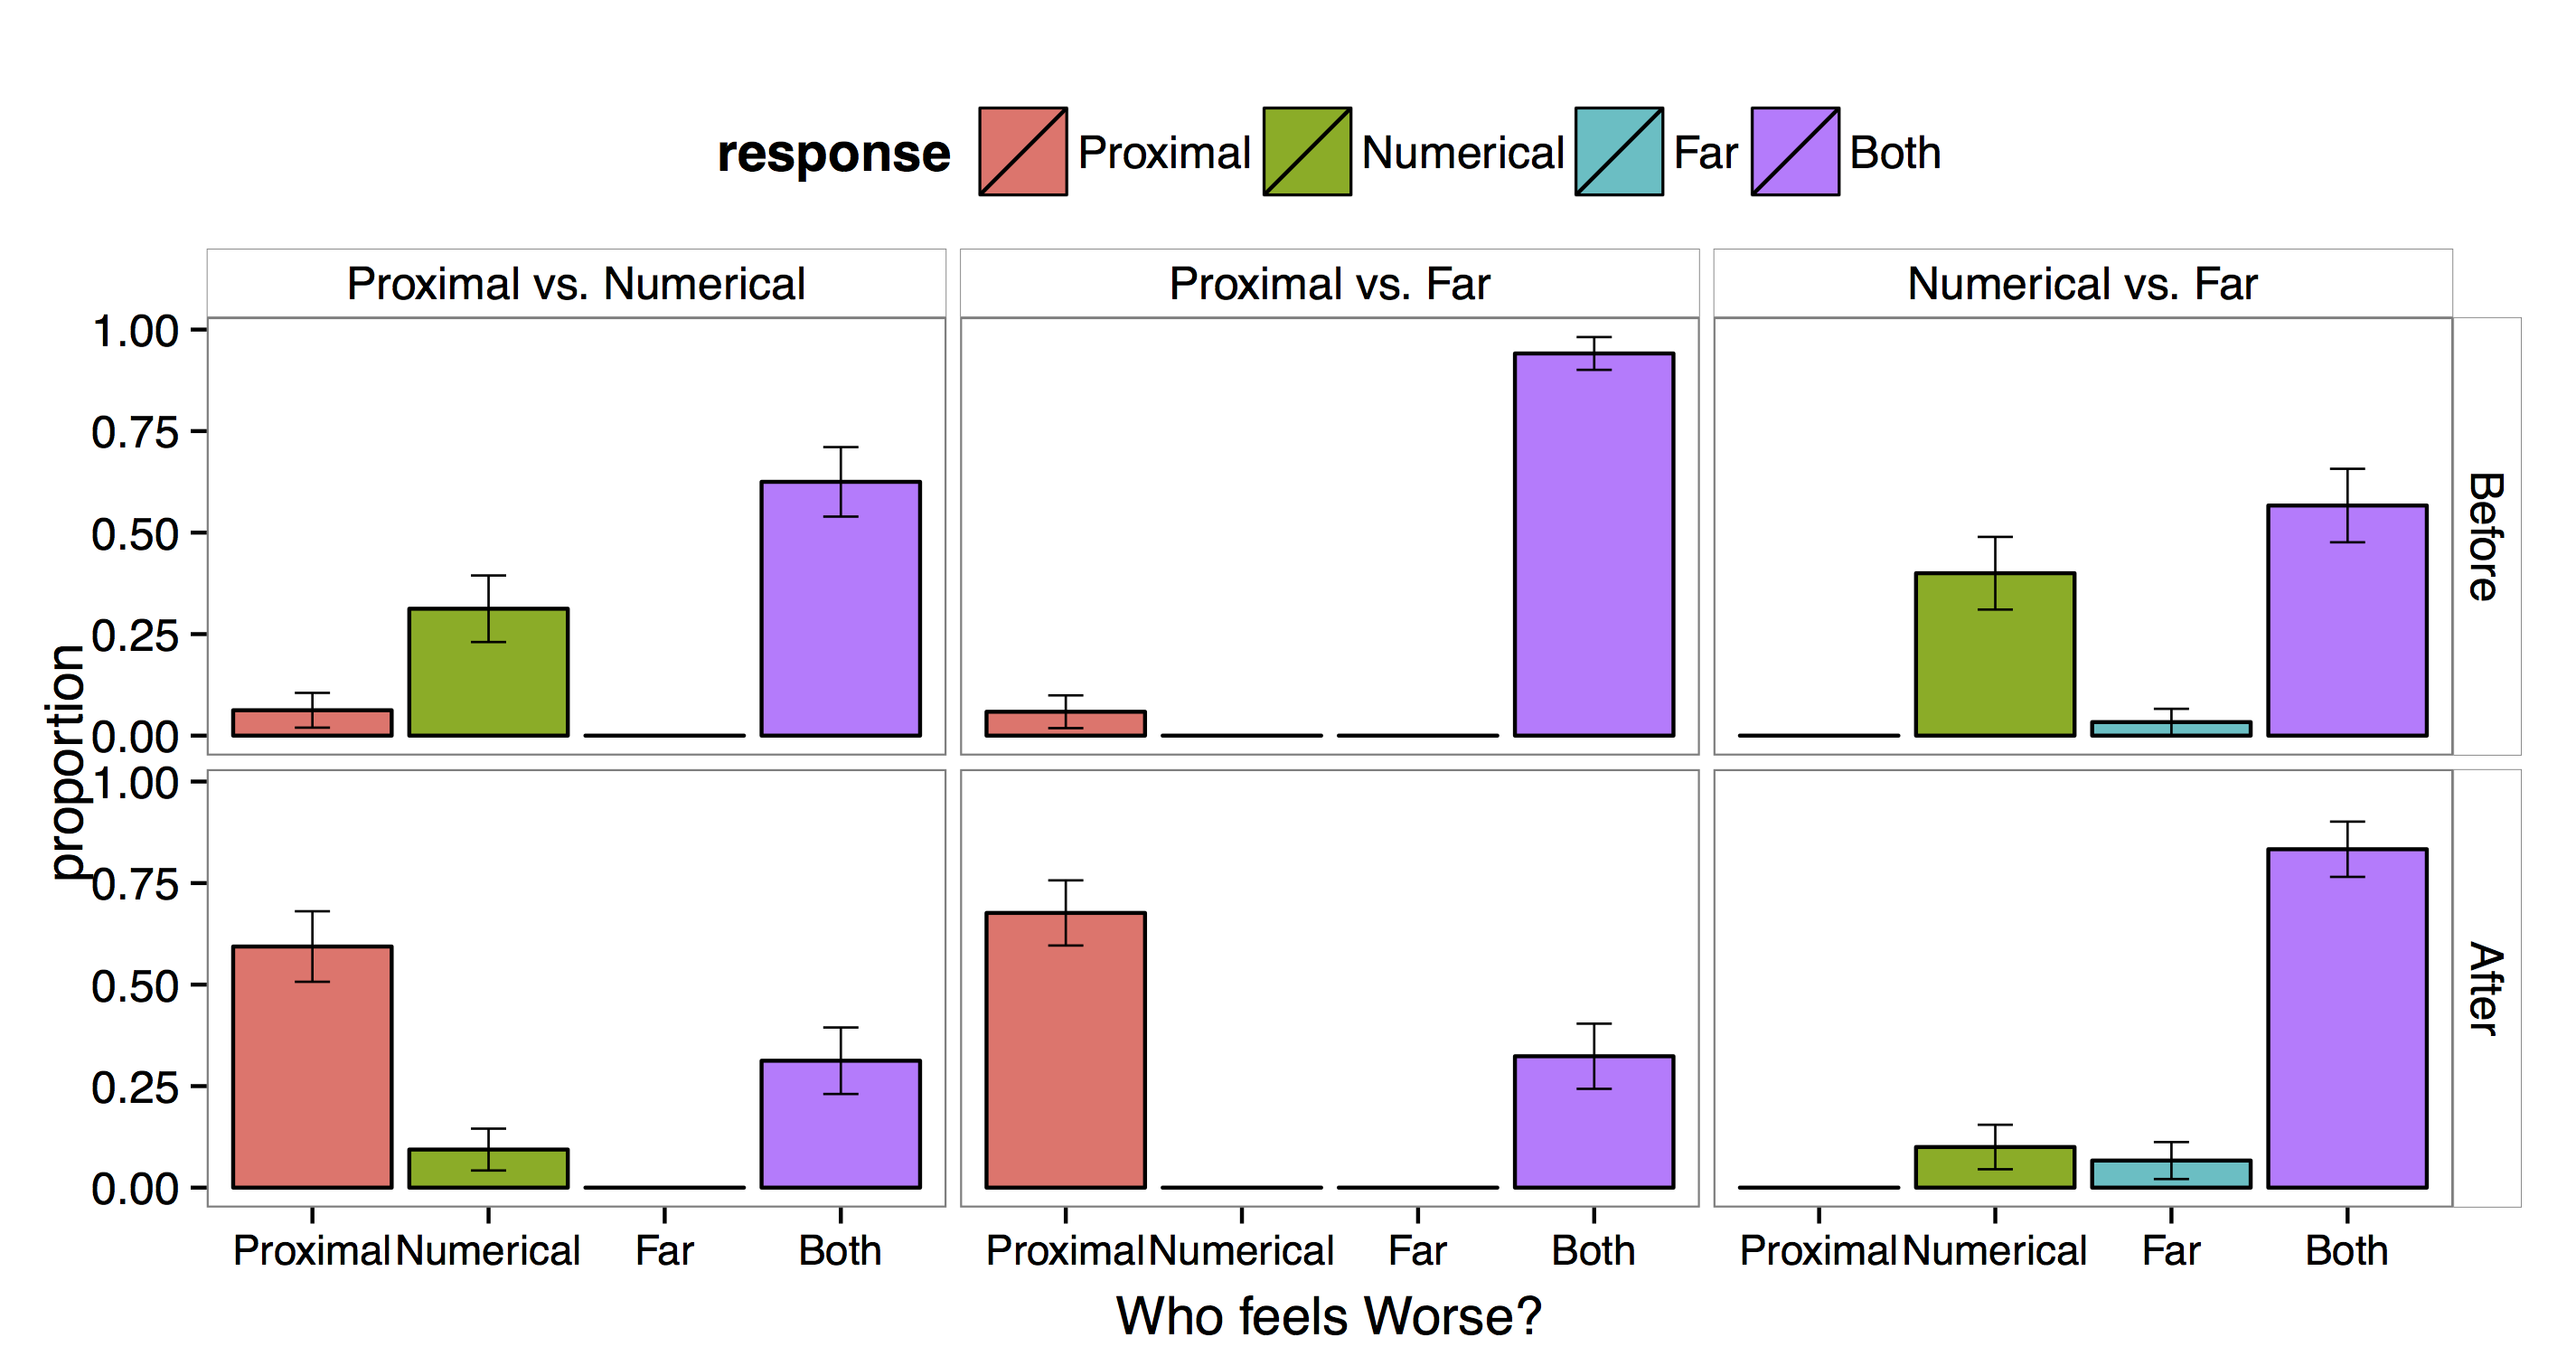
\includegraphics[width=\columnwidth]{images/card_forcedWorse.png}
\caption{ Expt 3 Results. Will make this bigger.}
\label{Expt3ResultFig}
\end{figure}



%
%In particular, there are 2 main questions that a model should answer:
%How are different types of distances related?
%
%Missing a plane by 5 minutes versus 30 \cite{Kahneman1982}
%
%Missing a goal in soccer by 5 inches versus 30
%
%Entering a store just ahead of a person who won a prize for being the one-millionth customer \cite{Roese1997}
%
%A �near miss� on a slot machine (e.g., Clark, Lawrence, Astley-Jones, \& Gray, 2009)
%
%In a game where one has to roll a 6 on a die to win, rolling a 5 versus rolling a 2 \cite{Kahneman1990}
%
%How do these distances factor (quantitatively) into our affective judgments?
%
%Here, I propose a model of a lay theory of counterfactual distance, a distance measure to the counterfactual world, and in particular, how counterfactual distance might factor into the affective judgments that human observers make about possible counterfactual worlds. These distances---temporal distance; physical distance; semantic distance in some mental representation space; etc---measure the separation between the current world and the counterfactual world being considered. The model proposes how observers consider these other possible worlds and details the affective impact that counterfactual distance has. 



\section{Acknowledgments}

This work was supported in part by an A*STAR National Science Scholarship to DCO and by a James S. McDonnell Foundation Scholar Award to NDG.


\bibliographystyle{apacite}

\setlength{\bibleftmargin}{.125in}
\setlength{\bibindent}{-\bibleftmargin}

\bibliography{cfDistance}


\end{document}
